\chapter{Analisis}
\label{chap: analisis}

\section{Analisis Data Penilaian Skripsi}
\label{sec: analisisData}

	Berdasarkan analisa dari contoh form penilaian skripsi yang ada, dapat disimpulkan bahwa penilaian skripsi membutuhkan data-data sebagai berikut:
		
		\begin{enumerate}
			\item Semester
			\item Tahun ajaran
			\item NPM mahasiswa 
			\item Nama mahasiswa
			\item Judul skripsi
			\item Nama pembimbing utama/tunggal
			\item Nama pembimbing pendamping(tidak harus)
			\item Nama ketua tim penguji
			\item Nama anggota tim penguji
			\item Bobot ketua tim penguji
			\item Bobot anggota tim penguji
			\item Bobot pembimbing
			\item Nilai koordinator skripsi
			\item Bobot koordinator skripsi
			\item Bobot tata tulis laporan ketua
			\item Bobot kelengkapan materi ketua
			\item Bobot penguasaan materi ketua
			\item Bobot presentasi ketua
			\item Bobot pencapaian tujuan ketua
			\item Bobot tata tulis laporan anggota
			\item Bobot kelengkapan materi anggota
			\item Bobot penguasaan materi anggota
			\item Bobot presentasi anggota
			\item Bobot pencapaian tujuan anggota
			\item Bobot tata tulis laporan pembimbing
			\item Bobot kelengkapan materi pembimbing
			\item Bobot penguasaan materi pembimbing
			\item Bobot bimbingan pembimbing
			\item Nilai akhir mahasiswa
		\end{enumerate}
	
	Berdasarkan diskusi dengan dosen pembimbing, disimpulkan bahwa sistem penilaian sidang skripsi 2 ini hanya memerlukan penyimpanan untuk bobot masing-masing penilaian dan nilai akhir mahasiswa untuk tahap perhitungan. Hal ini dikarenakan nilai-nilai lainnya dapat dihasilkan dengan melakukan perhitungan pada  nilai akhir mahasiswa dan bobot nilai yang diinginkan. Begitu pula dengan nilai dari masing-masing penguji.
	
		\begin{figure}[H]
			\centering
			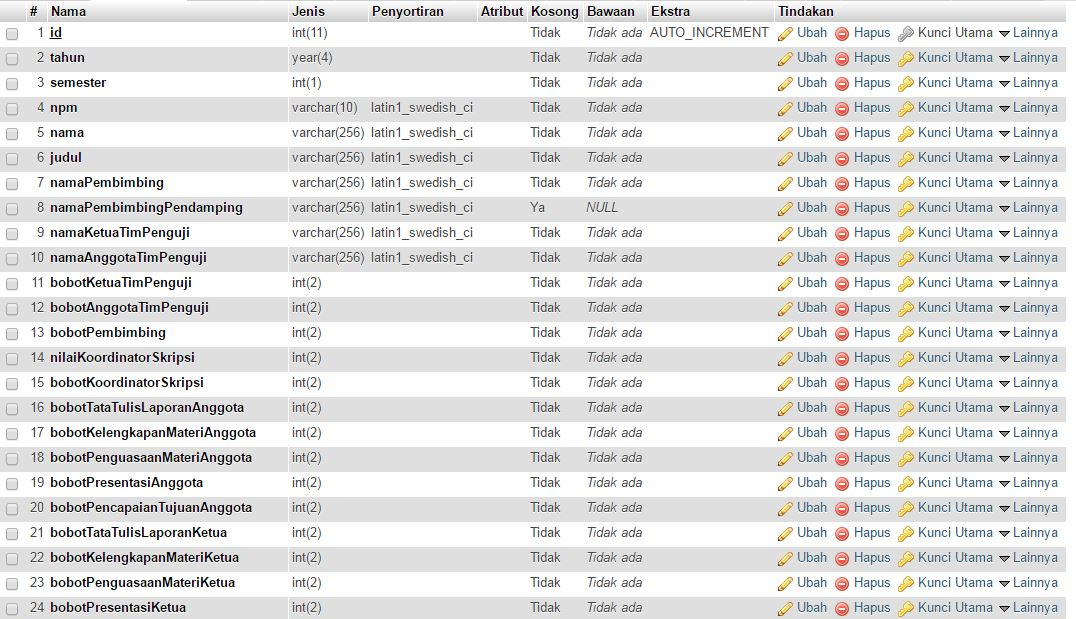
\includegraphics[scale= 1.0]{Gambar/database1}
			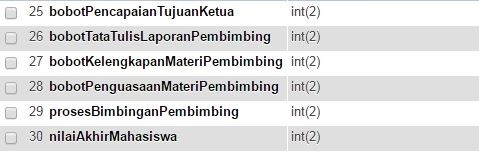
\includegraphics[scale= 1.0]{Gambar/database2}
			\caption {Data yang disimpan di database}
			\label{fig:tabeldata}
		\end{figure}
	
\section{Analisis Tampilan Sistem Informasi Penilaian Skripsi}
\label{sec: analisisTampilan}
	
	Tampilan pada sistem informasi penilaian skripsi haruslah dibuat semirip mungkin dengan form penilaian skripsi yang sudah ada seperti pada lampiran gambar \ref{fig: skripsiAsli} dan gambar \ref{fig: rekapAsli}.
	
	Perbedaan yang akan ditampilkan adalah dengan adanya otomatisasi penghitungan nilai sesuai dengan bobot yang diberikan kepada penilai. Hal ini akan memberikan kemudahan penilai untuk melakukan penilaian.
	
	Gambar \ref{fig:tampilan} adalah bayangan awal tampilan untuk sistem informasi penilaian skripsi:
	\begin{figure}[H]
		\centering
		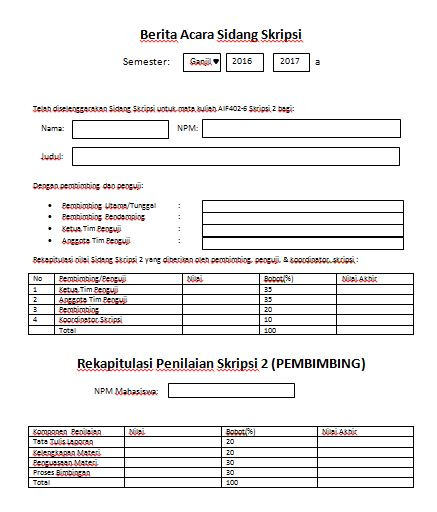
\includegraphics[scale=0.75]{Gambar/tampilan1}
		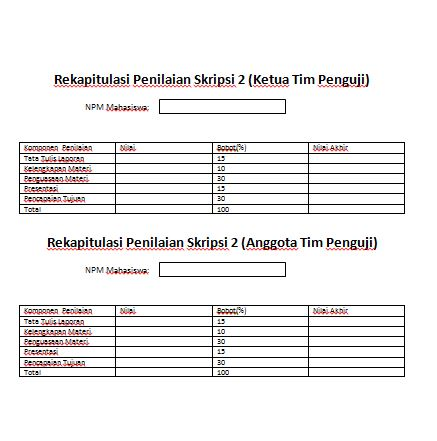
\includegraphics[scale=0.75]{Gambar/tampilan2}
		\caption{Perkiraan Tampilan}
		\label{fig:tampilan}
	\end{figure}
	
	Dari bayangan awal itulah, saya mendesain tampilan dari aplikasi sistem informasi penilaian skripsi 2 ini. Gambar \ref{fig:tampilanapp} merupakan tampilan pada aplikasi sistem informasi penilaian skripsi 2.
	
	\begin{figure}[H]
		\centering
		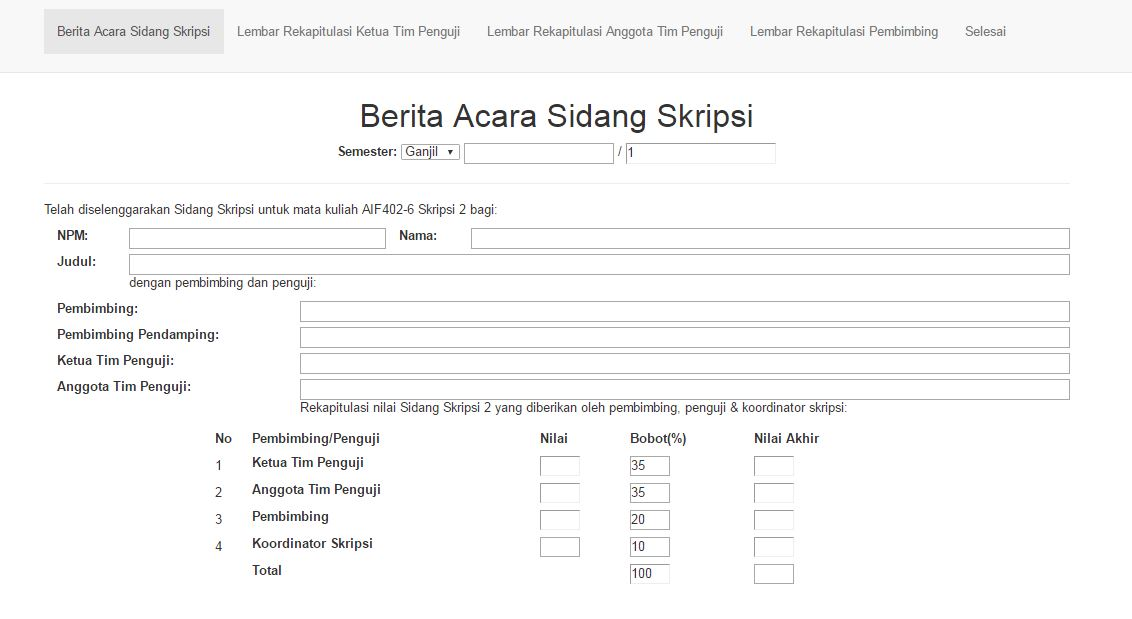
\includegraphics[scale=0.5]{Gambar/tampilanapp1}
		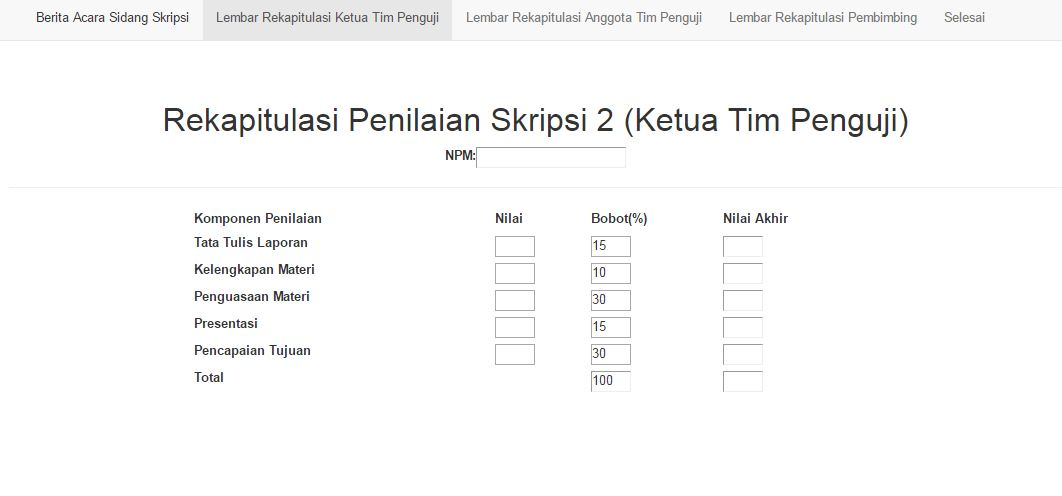
\includegraphics[scale=0.5]{Gambar/tampilanapp2}
		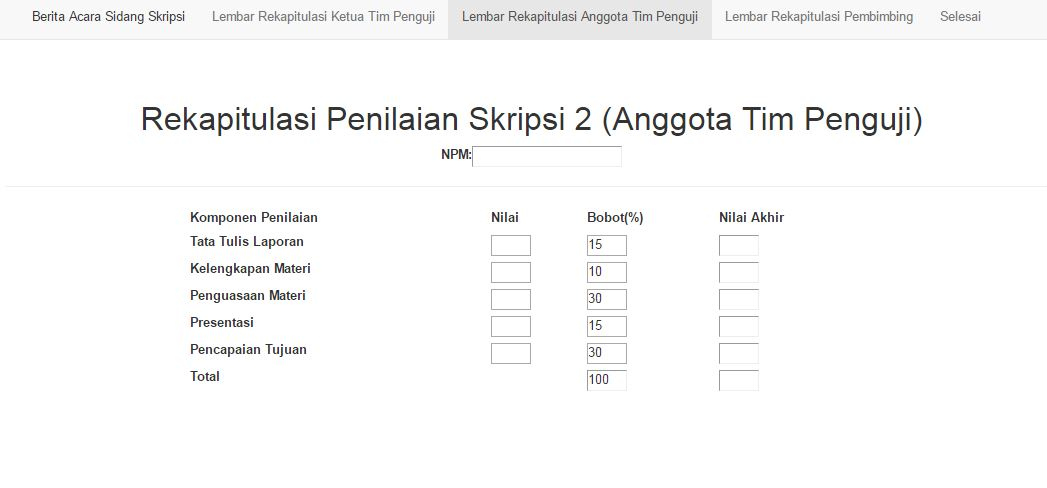
\includegraphics[scale=0.5]{Gambar/tampilanapp3}
		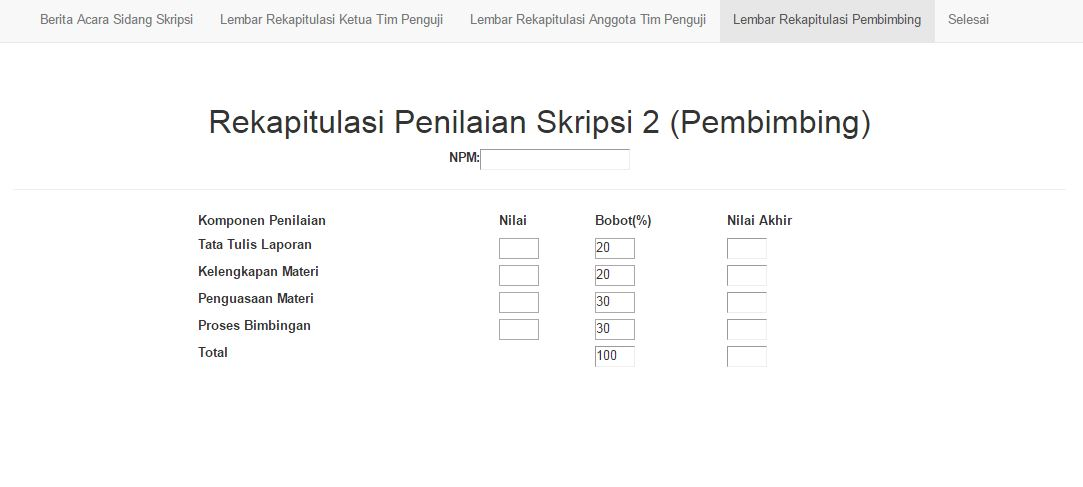
\includegraphics[scale=0.5]{Gambar/tampilanapp4}
		\caption{Perkiraan Tampilan}
		\label{fig:tampilanapp}
	\end{figure}